\documentclass[aspectratio=169]{beamer}

% SETUP =====================================
\usepackage[T1,T2A]{fontenc}
\usepackage[utf8]{inputenc}
\usepackage[russian]{babel}
\usepackage{hyperref}
\usepackage{listings}
\usepackage{array}
\usepackage{amssymb}
\usepackage{pifont}
\usepackage{../../beamerthemeslidesgeneric}
% SETUP =====================================

\title{Scala Object System}
\author{Mikhail Mutcianko, Alexey Otts}
\institute{СПБгУ, СП}
\date{\today}

\begin{document}

\frame{\titlepage}

\section{Recap: Syntax Differences from Kotlin}

\begin{frame}{Syntax}
  \centering
  \begin{tabular}{>{\ttfamily}r@{\ $\Leftrightarrow$\ }>{\ttfamily}l}
    Kotlin & Scala \\
    \hline
    \pause
    List<Integer> & List[Int] \\
    \pause
    fun foo(x: Integer): A \{ \} & def foo(x: Int): A = \{  \} \\
    \pause
    import foo.* & import foo.\_ \\
    \pause
    when(x) \{  \} & x match \{  \} \\
    \pause
    class Foo : Bar & class Foo extends Bar \\
    \pause
    -> & => \\
    \pause
    it & \_
  \end{tabular}
\end{frame}

\section{Scala Type System}

\begin{frame}{Everything is a type}
  \centering
  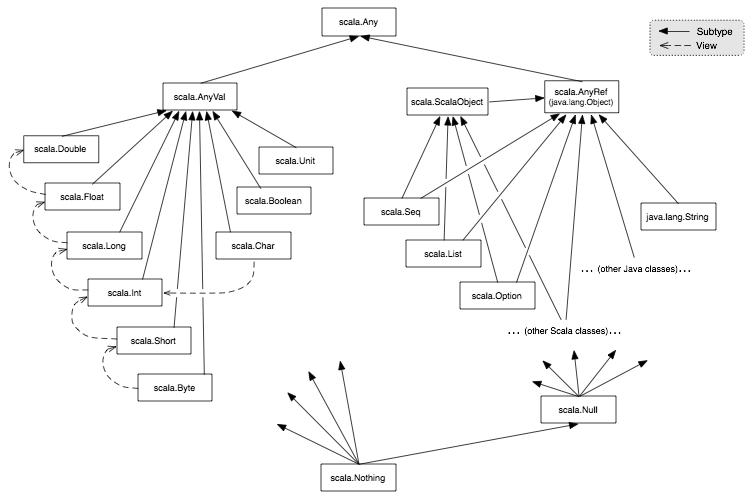
\includegraphics[scale=0.35]{classhierarchy.png}
\end{frame}

\begin{frame}{Top types}
\begin{itemize}
  \item \texttt{Any}
    \begin{itemize}
      \item The base type of all types
      \item Methods: \texttt{==, !=, equals, hashCode, toString}
    \end{itemize}
    \pause
  \item \texttt{AnyRef}
    \begin{itemize}
      \item The base type of all reference types
      \item Alias of \texttt{java.lang.Object}
    \end{itemize}
    \pause
  \item \texttt{AnyVal}
    \begin{itemize}
      \item The base type of all primitive types
    \end{itemize}
\end{itemize}
\end{frame}

\begin{frame}{Bottom type}
 \texttt{Nothing} is at the bottom of Scala's type hierarchy. It is a subtype of every other type.\\
 There is no value of type \texttt{Nothing}.
 \vspace{2em}
 \begin{block}{Why is that useful?}
   \begin{itemize}
     \item To signal abnormal termination
     \item As an element type of empty collections
   \end{itemize}
 \end{block}
\end{frame}

\section{Classes, Objects, Traits \ldots}

% basic
\begin{frame}[fragile]{Basic}
  \begin{lstlisting}[style=scala,language=scala]
class Useless

class Calculator {
  val brand: String = "HP"
  def add(m: Int, n: Int): Int = m + n
}
  \end{lstlisting}
\end{frame}

% class ctor
\begin{frame}{Class constructor}
  \begin{itemize}
    \item In Scala, a class implicitly introduces a primary constructor
    \item Takes the parameters of the class
    \item Executes all statements in the class body
    \item Can introduce members if parameters are specified as \texttt{val} or \texttt{var}
  \end{itemize}
\end{frame}

\begin{frame}[fragile]{Class constructor}{Example}
\begin{lstlisting}[style=scala,language=scala]
class Calculator(brand: String) {
  /*  A constructor  */
  val colour: String = if (brand == "TI") {
    "blue"
  } else if (brand == "HP") {
    "black"
  } else {
    "white"
  }
  def add(m: Int, n: Int): Int = m + n
}
\end{lstlisting}
\end{frame}

\begin{frame}[fragile]{Auxiliary Constructors}
  \begin{block}{}
    Scala also allows the declaration of auxiliary constructors.\\
    These are methods named \texttt{\alert{this}} 
  \end{block}
 \vspace{1em}
\begin{lstlisting}[style=scala,language=scala]
class Calculator(brand: String) {
  val color: String = ???

  def this(other: Cal) = ??? // <<<

  // An instance method.
  def +(m: Int, n: Int): Int = m + n
}
\end{lstlisting}
\end{frame}

% no statics - objects
\begin{frame}{Objects}
  \begin{itemize}
    \item Scala has no static classes / methods / fields
    \item Objects are used to hold single instances of a class
    \item Objects are lazy, and are not initialized until first reference
  \end{itemize}  
\end{frame}

\begin{frame}[fragile]{Objects}{Example}
\begin{lstlisting}[style=scala,language=scala]
object Constants {
  val e = 2.71828182846
  def **(num: Double) = num * e
}

Constants ** Constants.e
\end{lstlisting}
\end{frame}

% companion objects
\begin{frame}[fragile]{Companion objects}
\begin{block}{}
  A companion object in Scala is an object that’s declared in the same file as a class, and has the
  same name as the class
\end{block}
 \vspace{1em}
\begin{lstlisting}[style=scala,language=scala]
class SomeClass {
    def printFilename() = {
        println(SomeClass.HiddenFilename)
    }
}

object SomeClass {
    private val HiddenFilename = "/tmp/foo.bar"
}
\end{lstlisting}
\end{frame}

% traits and abstract classes
\begin{frame}{Traits}
  \begin{block}{}
    Traits are collections of fields and behaviors that you can extend or mixin to your classes
  \end{block}
  \begin{itemize}
    \item In Scala, a class can only have one superclass, but many traits
    \item Can have methods and properties
    \item \alert{Can have} member definitions
    \item Cannot have constructors
  \end{itemize}
\end{frame}

\begin{frame}[fragile]{Traits}{Example}
\begin{lstlisting}[style=scala,language=scala]
trait Planar {
  def height: Int
  def width: Int
  def surface = height * width // <<<
}

class Square extends Shape with Planar with Movable
\end{lstlisting}
\end{frame}

% abstract classes
% binary compatibility of traits ?
\begin{frame}{Abstarct classes}
  \begin{itemize}
    \item Can have methods and properties
    \item Can have member definitions
    \item \alert{Can} have constructors
  \end{itemize}
\end{frame}

% super calls
\begin{frame}{Super calls}
  \begin{block}{Problem}
    To keep your Scala code DRY (“Don’t Repeat Yourself ”), you want to invoke a method that’s
    already defined in a parent class or trait.
  \end{block}
\end{frame}

\begin{frame}[fragile]{Super calls}{Example}
\begin{lstlisting}[style=scala,language=scala]
class WelcomeActivity extends Activity {
    override def onCreate(bundle: Bundle) {
        super.onCreate(bundle)
        // more code here ...
    }
}
\end{lstlisting}
\end{frame}

\begin{frame}[fragile]{Super calls}{Controlling which trait you call a method from}
\begin{lstlisting}[style=scala,language=scala]
class Child extends Human with Mother with Father {
    def printSuper = super.hello
    def printMother = super[Mother].hello
    def printFather = super[Father].hello
    def printHuman = super[Human].hello
}
\end{lstlisting}
\end{frame}

% properties and defs
\begin{frame}{Members}
\begin{itemize}
  \item \texttt{def} - method
  \item \texttt{val} - immutable property
  \item \texttt{var} - mutable property
  \item \texttt{lazy val} - lazy immutable property
\end{itemize}
\end{frame}

\begin{frame}{Properties}
  \begin{block}{}
    All properties \alert{implicitly} generate a backing field, a setter and a getter \\
    Except for \texttt{private} ones
  \end{block}
\end{frame}

\begin{frame}[fragile]{Properties}
\begin{lstlisting}[style=scala,language=scala]
class Person() {
 private var name = ""
 var age = 0
}
\end{lstlisting}
\pause
\begin{lstlisting}[style=scala,language=scala]
class Person() {
 private var name = ""
 // Private age variable, renamed to _age
 private var _age = 0

 // Getter
 def age = _age

 // Setter
 def age_= (value:Int):Unit = _age = value
}
\end{lstlisting}
\end{frame}

\begin{frame}{Concrete member overriding}
  \begin{columns}
    \begin{column}{0.5\textwidth}
      \begin{itemize}
        \item \texttt{val}: can only be overridden by val
        \item \texttt{lazy val}: can only be overridden by lazy val
        \item \texttt{var}: a concrete var cannot be overridden
        \item \texttt{def}: can be overridden by all kinds of members
      \end{itemize} 
    \end{column}
    \begin{column}{0.5\textwidth}
      \centering
      \begin{tabular}{|c|c|c|c|c|}
        \hline
         & val & lazy & var & def \\
        \hline
        val & \cmark & \xmark & \xmark & \xmark \\
        \hline
        lazy & \cmark & \xmark & \xmark & \xmark \\
        \hline
        var & \xmark & \xmark & \xmark & \xmark \\
        \hline
        def & \cmark & \cmark & \cmark & \cmark \\
        \hline
      \end{tabular}
    \end{column}
  \end{columns}
\end{frame}

\begin{frame}{Abstract member overriding}
  \begin{columns}
    \begin{column}{0.5\textwidth}
      \begin{itemize}
        \item \texttt{lazy val}: cannot be abstract
        \item \texttt{val}: can be overridden by val and lazy val
        \item \texttt{var}: can be overridden by var, or a pair of read and write operations
          implemented by def, val, or lazy val
        \item \texttt{def}: can be overridden by all kinds of members
      \end{itemize} 
    \end{column}
    \begin{column}{0.5\textwidth}
      \centering
      \begin{tabular}{|c|c|c|c|}
        \hline
         & val & var & def \\
        \hline
        val & \cmark  & \xmark & \xmark \\
        \hline
        var & \cmark+  & \cmark & \cmark+ \\
        \hline
        def & \cmark  & \cmark & \cmark \\
        \hline
      \end{tabular}
    \end{column}
  \end{columns}
\end{frame}

% access modifiers
\begin{frame}{Acess modifiers}
  \begin{block}{Problem}
    Scala methods are public by default, and you want to control their scope in ways similar to
    Java.
  \end{block}
  \pause
  \begin{block}{Scopes}
    \begin{itemize}
      \item \alert<3>{object-private scope}
      \item private
      \item \alert<3>{package} 
      \item protected
    \end{itemize}
  \end{block}
\end{frame}

\begin{frame}[fragile]{Access modifiers}{object-private}
\begin{block}{}
The most restrictive access is to mark a method as “object-private.” When you do this, the method is
available only to the current instance of the current object. Other instances of the same class
cannot access the method.
\end{block}
\begin{lstlisting}[style=scala,language=scala]
class Foo {
    private[this] def isFoo = true
    def doFoo(other: Foo) {
        if (other.isFoo) {  // this line won't compile
            // ...
        }
    }
}
\end{lstlisting}
\end{frame}

\begin{frame}[fragile]{Access modifiers}{package scope}
\begin{lstlisting}[style=scala,language=scala]
package com.acme.coolapp.model {
    class Foo {
        private[model] def doX {}
        private def doY {}
    }
    class Bar {
        val f = new Foo
        f.doX  // compiles
        f.doY  // won't compile
    }
}
\end{lstlisting}
\end{frame}

% apply method
\begin{frame}{\texttt{apply} method}
  \texttt{apply} is a syntactic sugar for calling something
  \begin{itemize}
    \item construct new instances
    \item directly call anonymous functions
    \item mimic callable behaviour
    \item see also: \texttt{update} method
  \end{itemize}
\end{frame}

\begin{frame}[fragile]{\texttt{apply} method}{example}
\begin{lstlisting}[style=scala,language=scala]
class SomeClass(val x: Int)

object SomeClass {
  def apply(x: Int) = new SomeClass(x)
}

new SomeClass(42)
SomeClass(42)
\end{lstlisting}
\end{frame}

% imports
\begin{frame}[fragile]{Packages}
\begin{itemize}
  \item declare one or more package names at the top of a Scala file
    \begin{lstlisting}[style=scala,language=scala]
package users
class User
    \end{lstlisting}
    \pause
  \item declare packages by using braces
    \begin{lstlisting}[style=scala,language=scala]
package users {
  package administrators {
    class NormalUser
  }
  package normalusers {
    class NormalUser
  }
}
    \end{lstlisting}
\end{itemize}
\end{frame}

\begin{frame}[fragile]{Imports}
\begin{itemize}
\item single name
\begin{lstlisting}[style=scala,language=scala]
import users.User
\end{lstlisting}
\pause
\item all from package
\begin{lstlisting}[style=scala,language=scala]
import users._
\end{lstlisting}
\pause
\item only import selected names
\begin{lstlisting}[style=scala,language=scala]
import users.{User, UserPreferences}
\end{lstlisting}
\pause
\item rename imported member
\begin{lstlisting}[style=scala,language=scala]
import users.{UserPreferences => UPrefs}
\end{lstlisting}
\end{itemize}
\end{frame}

% package objects
\begin{frame}{Package objects}
\begin{block}{}
Scala provides package objects as a convenient container shared across an entire package
\end{block}
\pause
\begin{itemize}
  \item can contain arbitrary definitions
\pause
  \item can inherit from other classes and traits
\pause
  \item one package object per package
\pause
  \item should be placed in \texttt{package.scala}
\end{itemize}
\end{frame}

\begin{frame}[fragile]{Package obejcts}
\begin{lstlisting}[style=scala,language=scala]
package com.myapp
package object model {
  val MAGIC_NUM = 42 // field
  def echo(a: Any) { println(a) } // method
}
\end{lstlisting}
\pause
\begin{lstlisting}[style=scala,language=scala]
package com.myapp.model
class MainDriver {
  echo(42)
  echo(MAGIC_NUM)
}
\end{lstlisting}
\end{frame}

% early defs ?

\section{Functional OOP}

% Unapply method
\begin{frame}{Extractor object}
  \centering\large An extractor object is an object with an unapply method.
  \vspace{2em}
  \begin{columns}[T]
    \begin{column}{0.5\textwidth}
      \begin{block}{\texttt{apply}}
       takes arguments and creates an object
      \end{block} 
    \end{column}
    \begin{column}{0.5\textwidth}
      \begin{block}{\texttt{unapply}}
       takes an object and tries to give back the arguments
      \end{block} 
    \end{column}
  \end{columns}
\end{frame}

\begin{frame}{\texttt{unapply} method}{Return type}
  \begin{itemize}
    \item If it is just a test, return a \texttt{Boolean}
    \item If it returns a single sub-value of type \texttt{T}, return an \texttt{Option[T]}
    \item If you want to return several sub-values \texttt{T1,...,Tn,} group them in an optional tuple \texttt{Option[(T1,...,Tn)]}
  \end{itemize}
\end{frame}

\begin{frame}[fragile]{Extractor object}{Example}
\begin{lstlisting}[style=scala,language=scala]
class Cat(val name: String, val age: Int)

object Cat {
  def apply(name: String, age: Int): Cat = new Cat(name, age)
  def unapply(cat: Cat): Option[(String, Int)] = Some(cat.name -> cat.age)
}
\end{lstlisting}
\end{frame}

%\begin{frame}{Value class based extraction}{Zero allocation approach}

%\end{frame}

% ADTs - sealed traits
\begin{frame}{Sealed traits}
\begin{itemize}
  \item sealed traits can only be extended in the same file
    \pause
  \item this lets the compiler easily know all possible subtypes
    \pause
  \item example: the compiler can emit warnings if a match/case expression is not exhaustive
    \pause
  \item use sealed traits when the number of possibly subtypes is finite and known in advance
    \pause
  \item they can be a way of creating something like an enum in Java
    \pause
  \item they help you define algebraic data types, or ADTs
\end{itemize}
\end{frame}

\begin{frame}[fragile]{Sealed traits}{Example}
\begin{lstlisting}[style=scala,language=scala]
sealed trait Answer
case object Yes extends Answer
case object No extends Answer
case class  Maybe(something: String)
\end{lstlisting}
\end{frame}

% case classes & objects
\begin{frame}{Clase classes}
\begin{block}{}
  \texttt{Case classes} are used to conveniently store and match on the contents of a class. You can
  construct them without using \alert{new}
\end{block}
    \pause
Case classes auto generate:
\pause
\begin{itemize}
  \item properties based on constructor arguments
    \pause
  \item \texttt{equals}, \texttt{canEqual}, \texttt{hashCode} and \texttt{toString} based on properties
    \pause
  \item companion object with \texttt{apply} and \texttt{unapply} methods
    \pause
  \item \texttt{copy} method with default values
\end{itemize}
\end{frame}

% destructing assignment
\begin{frame}[fragile]{Destructuring bindings}
  \begin{block}{}
    Initializing a value may be more than binding a name --- it's a pattern.
  \end{block}
  \vspace{2em}
  \pause
\begin{lstlisting}[style=scala,language=scala]
val pi = 3.1415
val pi: Double = 3.1415   // equivalent to first definition
val c@Cat(name, age) = Cat("bobik", 42) // a pattern definition
val x :: xs = c :: name :: age :: Nil      // an infix pattern definition
\end{lstlisting}
\end{frame}

% pattern matching
\begin{frame}[fragile]{Pattern matching}{Values}
\begin{lstlisting}[style=scala,language=scala]
val times = 1

times match {
  case 1 => "one"
  case 2 => "two"
  case _ => "some other number"
}
\end{lstlisting}
\end{frame}

\begin{frame}[fragile]{Pattern matching}{Guards}
\begin{lstlisting}[style=scala,language=scala]
val times = 1

times match {
  case i if i == 1 => "one"
  case i if i == 2 => "two"
  case _ => "some other number"
}
\end{lstlisting}
\end{frame}

\begin{frame}[fragile]{Pattern matching}{Types}
\begin{lstlisting}[style=scala,language=scala]
val animal = Cat("eve", 10)

val owner = animal match {
  case a: Cat if a.name == "eve" => "Bob"
  case a: Dog if a.name == "dis" => "Mary"
  case _ => "Unknown"
}
\end{lstlisting}
\end{frame}

\begin{frame}[fragile]{Pattern matching}{Unapply}
\begin{lstlisting}[style=scala,language=scala]
val animal = Cat("eve", 10)

val owner = animal match {
  case Cat("eve", _) => "Bob"
  case Dog("dis", _) => "Mary"
  case _ => "Unknown"
}
\end{lstlisting}
\end{frame}

\begin{frame}[fragile]{Pattern matching}{Binding}
\begin{lstlisting}[style=scala,language=scala]
val animal = Cat("eve", 10)

val fullName = animal match {
  case c@Cat("eve", _) => s"Bob's ${c.name}"
  case d@Dog("dis", _) => s"Mary's ${d.name}"
  case _ => "Unknown"
}
\end{lstlisting}
\end{frame}

% functional list example

\section{Practice \\ Functional List}

%\section{Polymorphic Tyes}

% OOP polymorphism
% pattern matching and erasure
% type parameters
% subtyping relations
% variance
% sidenote: variance of java arrays
% variance for functions
% F-bound types

\end{document}

